In this chapter we describe our tool \liftcreate{}, which implements
the heuristic algorithm presented in the previous sections.
When considering the new approaches for their evaluation we shared the 
same encompassing environment and interface.
\liftcreate{} is a web-based application written in Java. To create
designs from specifications, the tool retrieves all the components 
data from a database of commercial parts from different suppliers
and explores the space of potential solutions guided by the user's
preferences. The interaction with the user allows to shape and refine
the heuristic search and pruning in the solutions space: the heuristic
procedure detailed in Algorithm~\ref{alg:hr} is geared towards
producing solutions as close as possible to human-conceived ones.

In practice, \liftcreate{} takes the designer from the very first
measurements and requirements, e.g., shaft size and payload, to a 
complete design which guarantees feasibility within a specific normative
framework. To achieve this, as first the user is asked to enter relevant
parameters characterizing the project and an overall goal to pursue.
For instance, if the size of the elevator's shaft is known and fixed
in advance, \liftcreate{} can generate solutions which maximize payload,
door size or car size. The goal is just a set of guidelines which, e.g.,
prioritize door size over other elements still keeping into account
the hard constraints.

\section{Software architecture}
\label{sec:arch-liftcreate}

\begin{figure}[t]
	\caption{\label{fig:elev_onto} Taxonomy of \liftcreate's elevator
		models (top) and details of the components of
		\texttt{OnePistonRopedHydraulicElevator} (bottom). Rectangles
		represent entities, IS-A relations are denoted by solid arrows, 
		and HAS-A relations are denoted by diamond-based arrows.} 
	\centering
	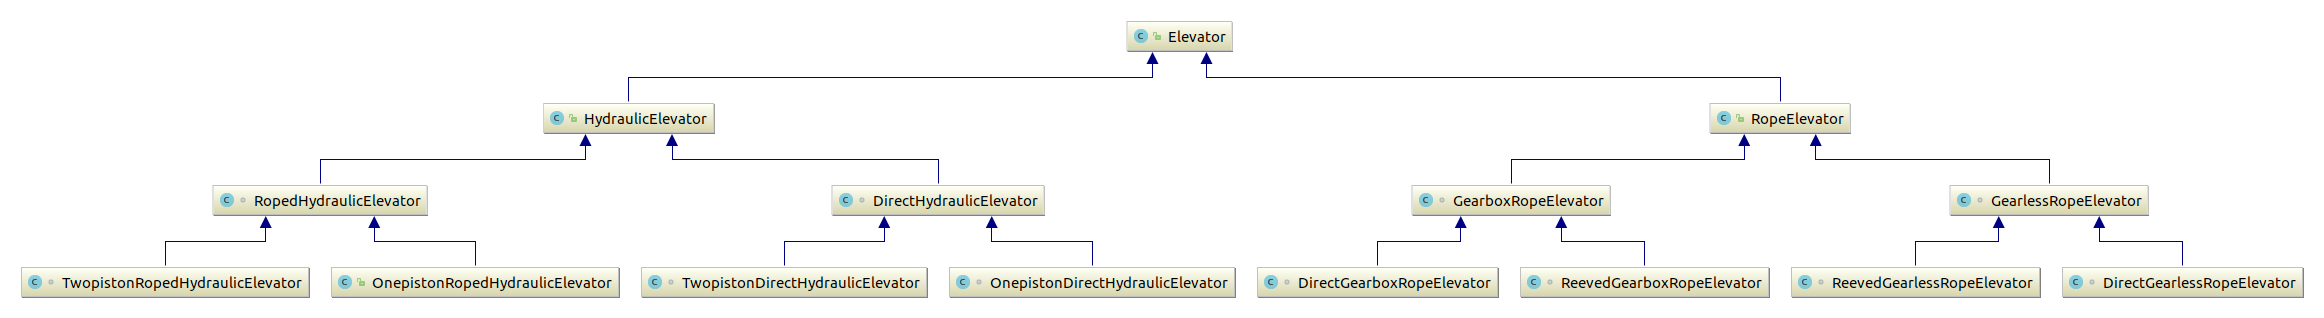
\includegraphics[width=\linewidth]{Elevator/ClassDiagramElevator.png}
	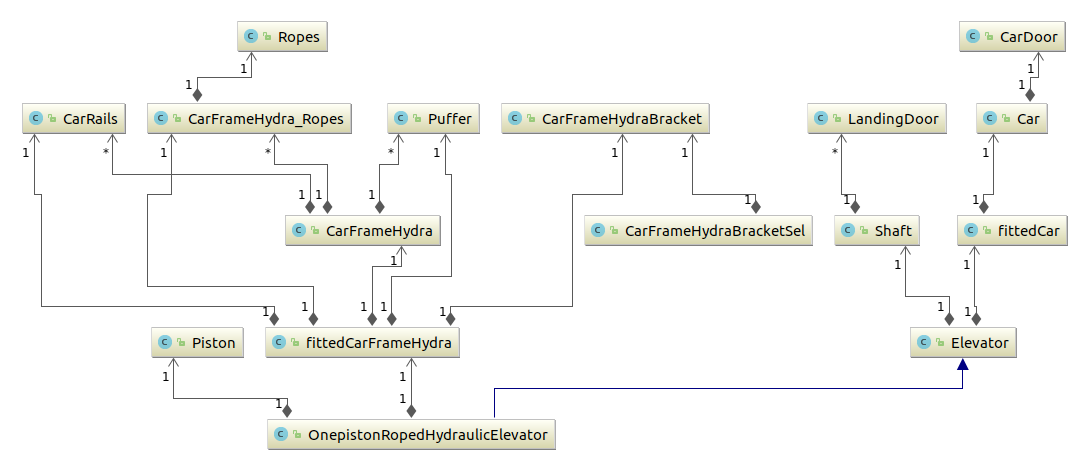
\includegraphics[width=.55\linewidth]{Elevator/ClassDiagramHydraulic.png}
\end{figure}

In order to manage the space of potential designs, \liftcreate{} does
not consider the RHEs components detailed in Section~\ref{sec:elevators}
solely as drawing elements, but they must be handled as first class data
inside the application logic. For example, \texttt{OnePistonRopedHydraulicElevator}
is both a leaf in the taxonomy shown in Figure~\ref{fig:elev_onto} (top)
and also the root node of the corresponding part-whole hierarchy (bottom).

Looking at the hierarchy, the structure of RHEs with one piston direct
drive can be easily learned, the only peculiar aspect being that these
implements feature only one piston (\texttt{Piston}). The remaining 
components are common to all \texttt{HydraulicElevator} or \texttt{Elevator}.
In particular, the car frame (\texttt{CarFrameHydra}), i.e., the mechanical
assembly connecting the car with the piston, is specific of hydraulics-powered
elevators. Albeit not physically part of the car frame, the entities
\texttt{CarRails}, i.e., the rails along which the car is constrained to
move, \texttt{Buffer}, i.e., the dumping device placed at the bottom of the
elevator shaft, and \texttt{Ropes}, are logically part of it since their 
type and size must be inferred from or melded with the type and size of the
car frame.

\begin{figure}
	\caption{\label{fig:sw-arch} Software architecture schema of \liftcreate.
		The three main modules reflect the Model-View-Controller pattern and
		are connected via REST calls.}
	\centering
	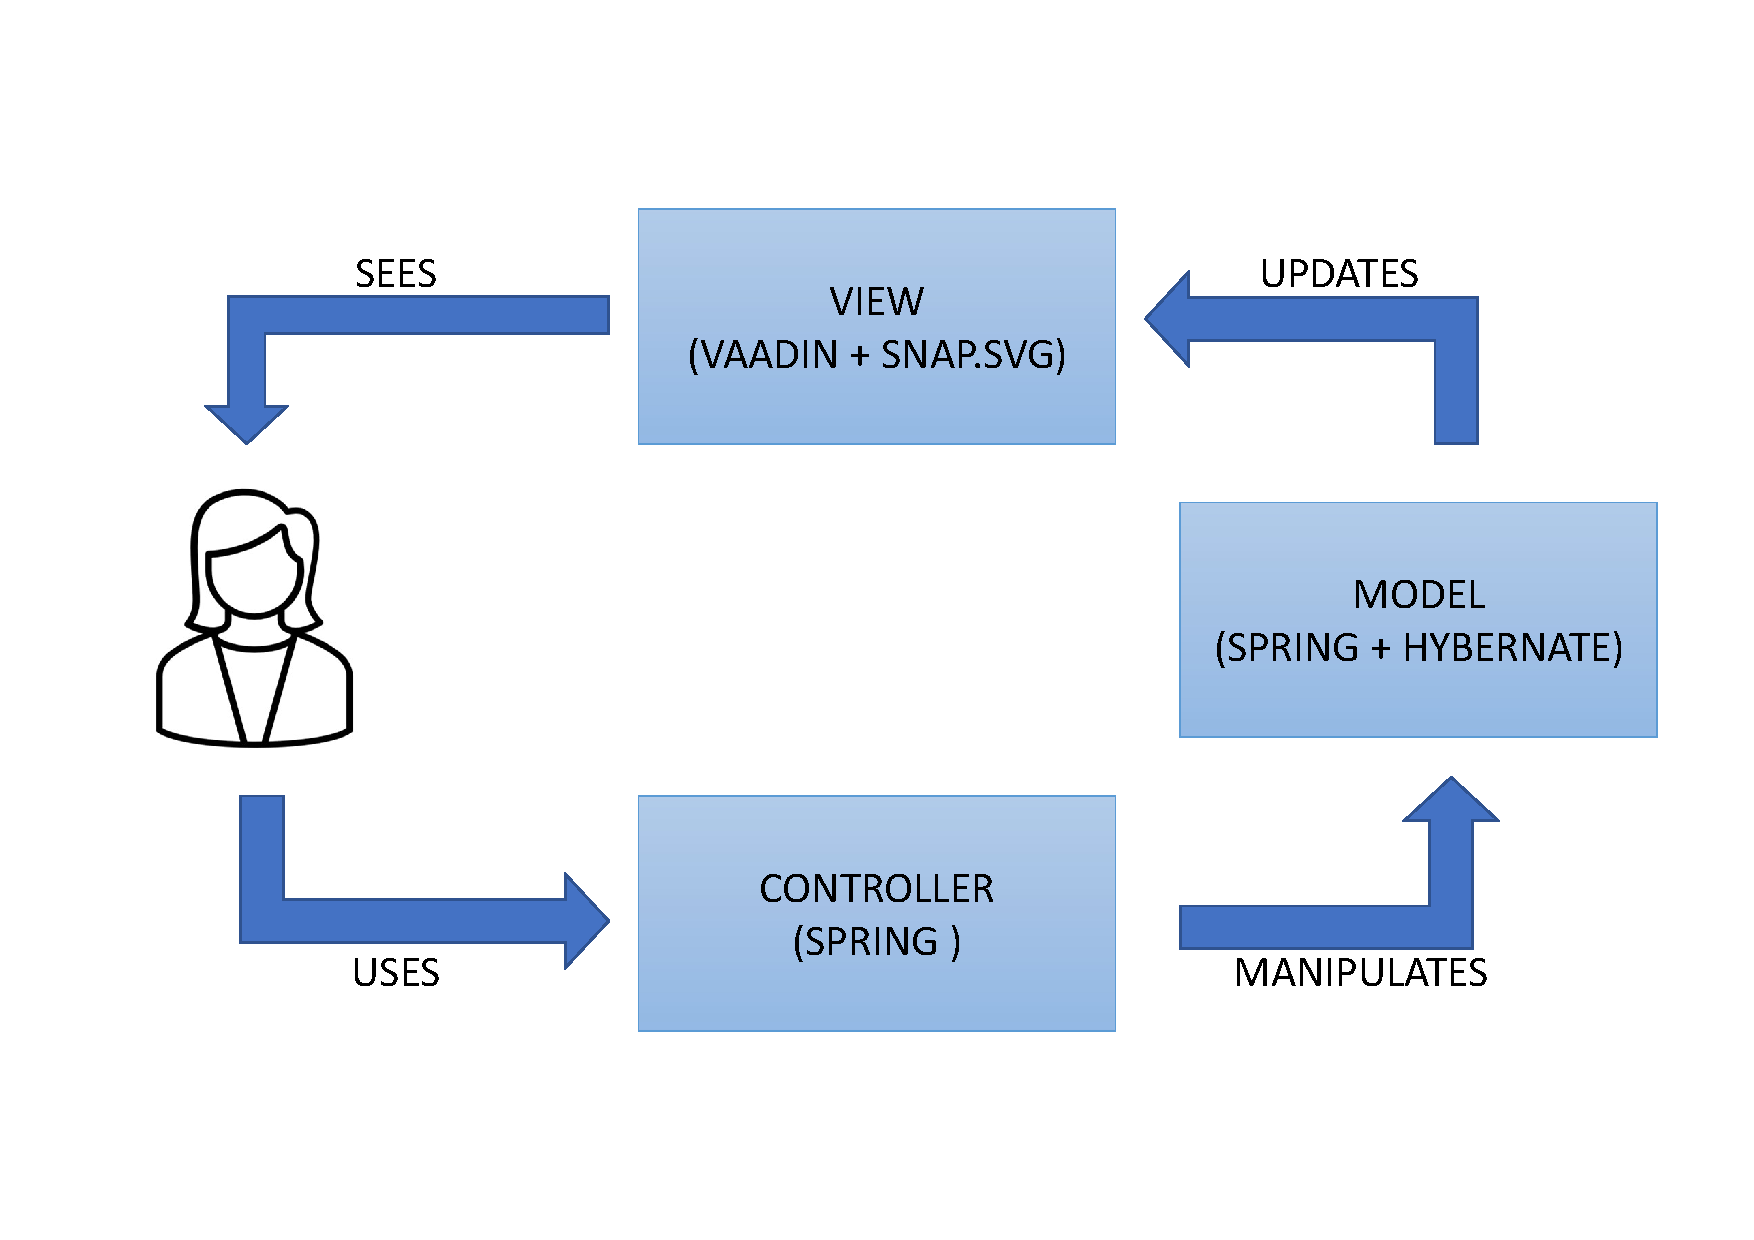
\includegraphics[width=.8\linewidth]{Elevator/SwArch.pdf}
\end{figure}

Common to all elevator types, the entities \texttt{Shaft} and \texttt{Car} are
both logically part of the \texttt{Elevator} entity, but only the \texttt{Car}
is also a physical component together with its sub-component \texttt{CarDoor}.
In the case of the \texttt{Shaft}, while landing doors (\texttt{LandingDoor})
are not physically part of it, they are attached to it and their size and type
must be inferred from or melded with car doors. The relationships encoded in
such part-whole hierarchy are instrumental to \liftcreate{} when it comes to
handle drawing, storage and retrieval of designs, but also to reason about
the various trade-offs of a design while searching in the space of potential
solutions.

\begin{figure}[t]
	\caption{\label{fig:liftcreate_1} Screenshot of \liftcreate's guidelines
		for generating designs. It is possible to select the vendor for the
		car frame mechanics as well as for the doors, and a further filter
		distinguishes between different door families.}
	\centering
	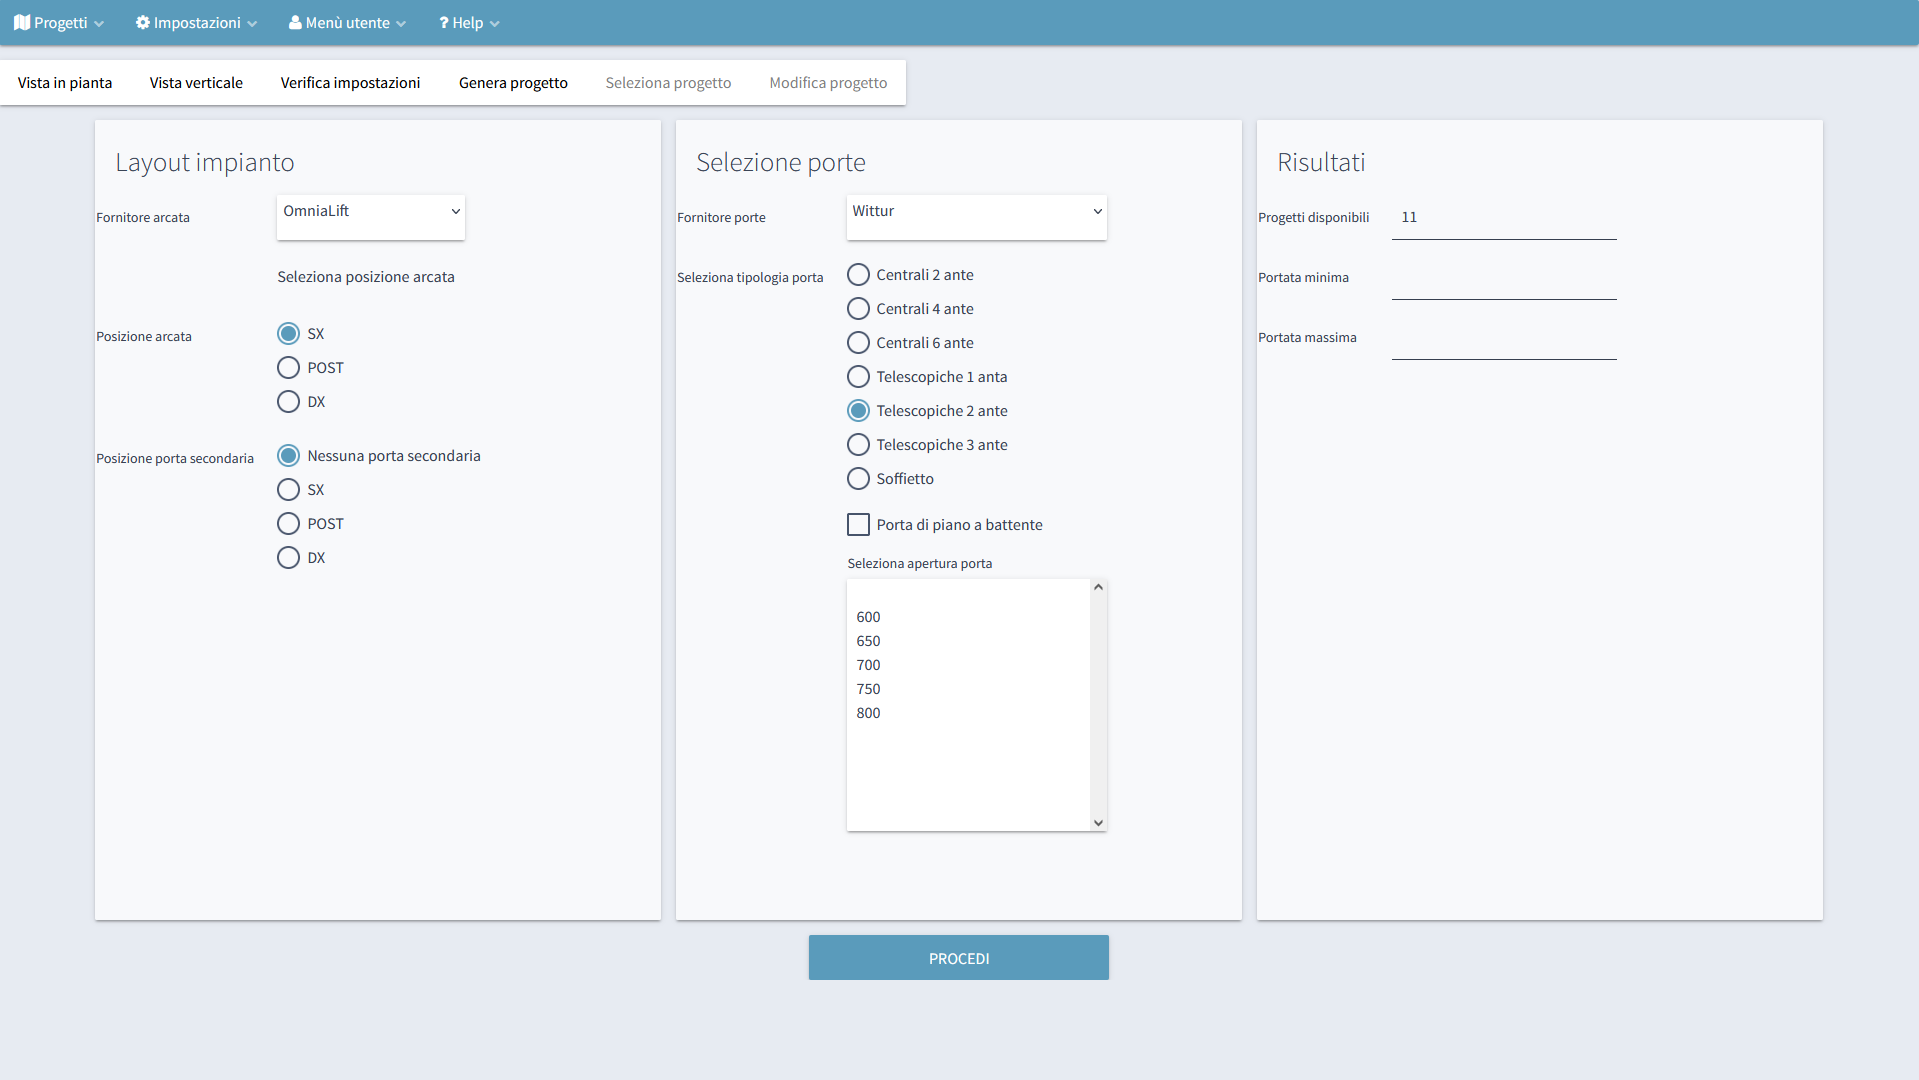
\includegraphics[width=\linewidth]{Elevator/DesignScreen.png}
\end{figure}

The heuristic configuration engine and the other approaches are developed as
REST services (REpresentational State Transfer), i.e., they exchange calls and
information with the client browser as JSON objects via HTTP. In this way, it
is possible to call a specific method by mapping an URL address supporting
GET and POST arguments. In Figure~\ref{fig:sw-arch} the schematic architecture 
following the Model-View-Controller (MVC) pattern is depicted. It divides the
related program logic in three interconnected elements and separates the internal
representations of information from the user's point of view.
The software is deployed server-side using the \textit{SPRING} Java framework, 
which is an asynchronous non-blocking architecture for developing and deploying 
web applications in a fast and secure way. We use this framework alongside with
\textit{Hybernate}, an Object Relational Mapping resource for achieving object 
persistence in the application and easily interchange the object representation
between SQL and Java.

\section{Web interface}
\label{sec:web_if}

\begin{figure}[t]
	\caption{\label{fig:liftcreate_2} Screenshot of a \liftcreate{} design
		obtained in the web application. On the left it is possible to see the
		alternative designs proposed.}
	\centering
	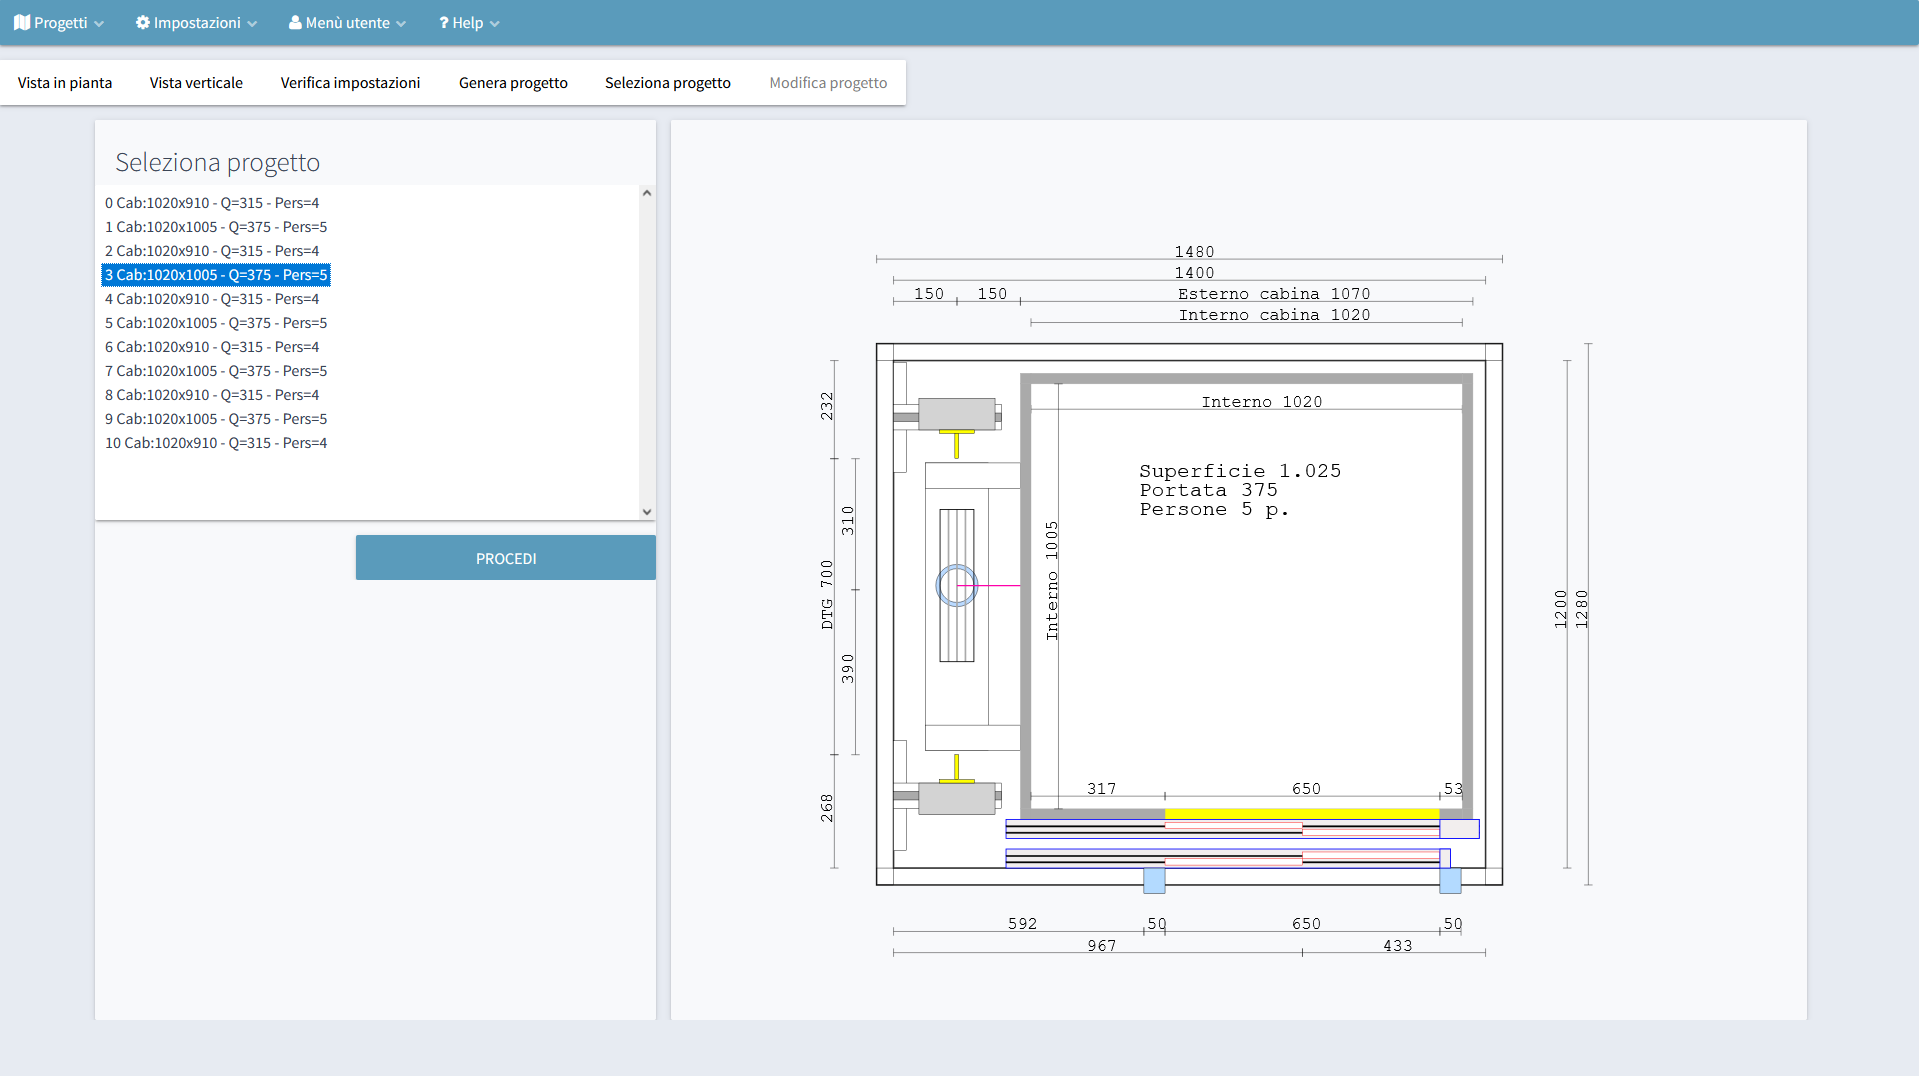
\includegraphics[width=\linewidth]{Elevator/PlanScreen.png}
\end{figure}

In order to build an interface which is fluent and interactive with the 
underlying logic, we build on the Java backend running the engine with the
VAADIN framework~\cite{vaadin14}. VAADIN allows us to incorporate 
the web interface in the same Java project, keeping available all the logic 
components and easing interaction between the user and the engine.

The web interface of \liftcreate{} is visible in Figures~\ref{fig:liftcreate_1}
and~\ref{fig:liftcreate_2}.
Figure~\ref{fig:liftcreate_1} is a screenshot of the heuristic engine
setup: here the user preferences are arranged in two areas.
First, the user chooses the elevator layout by selecting the car frame
vendor (\textit{Fornitore arcata}) and its position in the design 
(\textit{Posizione arcata}) --- the default position is on the left, 
and the main door is always at the bottom. Here the user can also 
request the placement of a second door (\textit{Posizione porta 
	secondaria}). Once the layout is chosen, the door selection tab
allows to further filter the solutions space by selecting $i$) the
door vendor (\textit{Fornitore porte}), $ii$) the door type
(\textit{Seleziona tipologia porta}) between symmetric, telescopic 
and folding with a different number of panels and $iii$) the door 
opening. This selection is actually evaluated in real time given the 
car frame and shaft measurements, filtering doors having an opening 
too big for the actual space.

In Figure~\ref{fig:liftcreate_2} we show the result of an example configuration
process, i.e., the output of the heuristic design generation. Once given the initial 
setting, \liftcreate{} presents a number of alternative designs --- 11, in this 
case --- matching the specifications. This is an extra feature that optimal 
approaches lack in principle, since they are designed to produce the single, 
best solution. The design is rendered in SVG and can be exported in the main 
formats for CAD users. The SVG includes all components and their dimensioning
in order to obtain a full-fledged CAD design. We manage to render the 
design --- and parts of it --- in the browser thanks to the Snap.svg~\cite{snap}
JavaScript library, that we use for wrapping custom components and arrange
them in the viewport. Note that Figure~\ref{img:planView} is a simplified and
clean version of the plan view generated by \liftcreate{} where we erased the
dimensioning. The top menu allows to fine-tune the general settings --- 
\textit{Impostazioni} --- by specifying the car wall thickness, the reductions,
i.e., the distance between the car walls and the shaft, and the safety margins.